\section{Introduction et présentation de l'étude\label{section:pres}}

\subsection{Introduction}

Dans les applications industrielles, dès lors que l'on travaille avec un écoulement dans un conduite chauffée, on peut se retrouver dans le cas d'un écoulement diphasique. Si la conduite est suffisamment longue, la prise en compte des pertes de charges risque d'être peu représentatif de la réalité, les pertes liées à l'ébullition n'étant pas négligeables.\\
Cette sous-estimation de la perte de pression lors du dimensionnement pourrait avoir des répercussions sur le rendement de l'installation ou bien la sécurité de celle-ci. Dans le cas d'un réacteur à eau pressurisé, il est important de connaître les conditions de l'écoulement à tous les endroits de la conduite. On ne souhaite pas se retrouver avec un fluide diphasique dans une zone où cela n'était pas prévu. Les conséquences pourrait être grave dans le cas d'une installation pour un réacteur nucléaire par exemple.


%Citer des applications utiles du calcul de perte de pression dans des écoulements diphasiques, exemples industriels, effet sur le rendement,catastrophes... 
\textcolor{red}{Parler des codes de calcul courants et des modèles existants}

\subsection{Présentation de l'étude}

Pour ce projet, nous nous intéressons à la perte de pression ainsi qu'au taux de vide moyen pour un écoulement bouillant dans une conduite chauffée. Une représentation d'un banc d'essai typique pour ce type de mesures est disponible à la fig. \ref{fig:instal}

\begin{figure}[htbp]
    \centering
    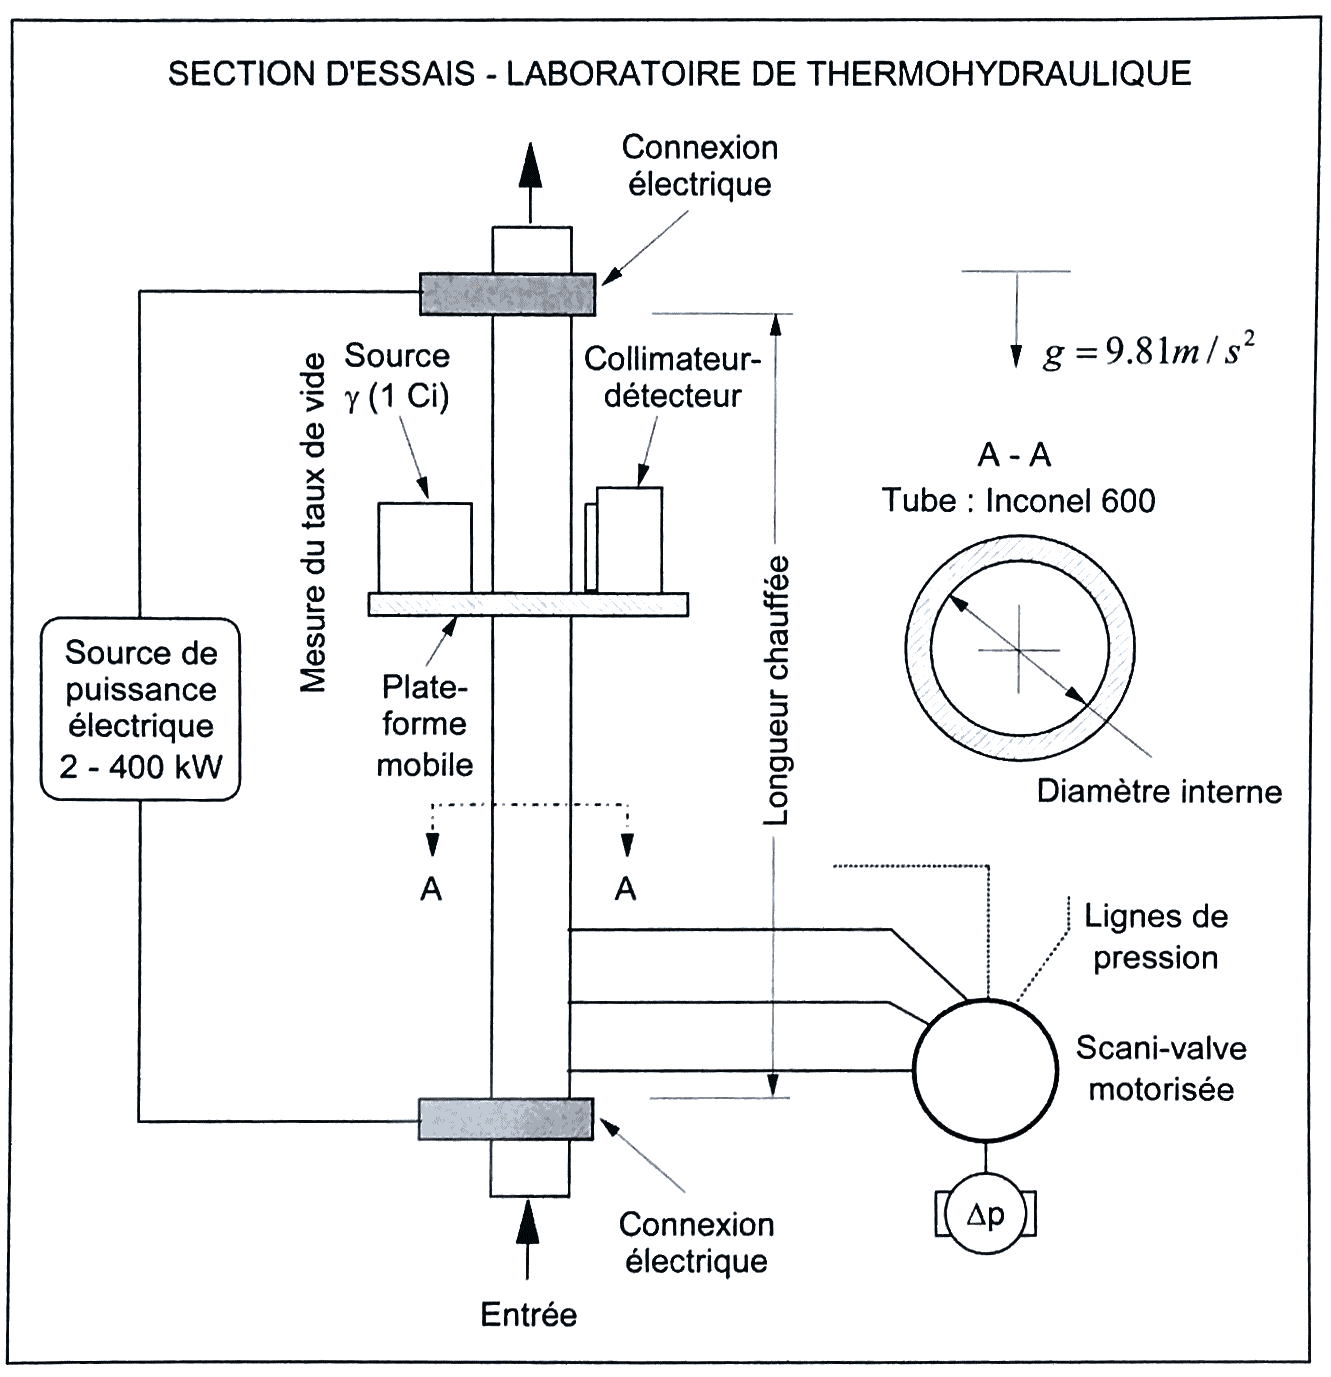
\includegraphics[width=0.8\textwidth]{images/schema_instal.png}
    \caption{Installation pour mesure de perte de pression et du taux de vide - D'après l'énoncé}
    \label{fig:instal}
\end{figure}

Le but de ce projet est de réaliser un modèle numérique et de déterminer les différents paramètres le long de la conduite. L'analyse des résultats se fait en comparant à des tables de données expérimentales. On travaille dans le cas d'un écoulement vertical ascendant.\\ \par
Pour réaliser cela, plusieurs hypothèses ont été réalisées :
\begin{itemize}
    \item \textbf{H1} : L'écoulement est incompressible.
    \item \textbf{H2} : La perte de pression par accélération dans la région non bouillante est négligeable.
    \item \textbf{H3} : La perte de pression totale est négligeable par rapport à la pression de l'écoulement.
    \item \textbf{H4} : L'enthalpie de l'eau sous-refroidie à une température donnée est égale à l'enthalpie de saturation de l'eau correspondant à cette température
\end{itemize}
\vspace{12pt}
\par
La détermination des propriétés thermodynamiques a été faite avec \texttt{pyXSteam}, qui est une librairie Python sur la base de \texttt{X-Steam} disponible sur Excel et Matlab.\\
Le titre et le taux de vide moyen sont déterminés à l'aide des corrélations de \textsc{Chexal-Lellouche}. Le multiplicateur diphasique ainsi que les facteurs de frottements qui servent au calcul de la perte de pression proviennent eux de la corrélation de \textsc{Friedel}.\\ \par





